\documentclass[conference]{IEEEtran}
\IEEEoverridecommandlockouts

\usepackage{cite}
\usepackage{amsmath,amssymb,amsfonts}
\usepackage{algorithmic}
\usepackage{graphicx}
\usepackage{textcomp}
\usepackage{xcolor}
\usepackage{booktabs}
\usepackage{tikz}
\usepackage{url}
\usetikzlibrary{positioning,arrows.meta,fit,backgrounds,shapes.geometric}

\def\BibTeX{{\rm B\kern-.05em{\sc i\kern-.025em b}\kern-.08em
    T\kern-.1667em\lower.7ex\hbox{E}\kern-.125emX}}

\begin{document}

\title{SwarmGen: Partitioning a Diffusion Pipeline Across Heterogeneous Edge Devices}

\author{
\IEEEauthorblockN{Sudarshan Sridhar}
\IEEEauthorblockA{Department of Computer and Information Science\\
University of Michigan-Dearborn\\
sudars@umich.edu}
\and
\IEEEauthorblockN{Varun Patel}
\IEEEauthorblockA{Department of Computer and Information Science\\
University of Michigan-Dearborn}
}

\maketitle

\begin{abstract}
We present SwarmGen, a system that partitions Stable Diffusion Turbo (SD-Turbo)
across three heterogeneous edge devices: a Raspberry Pi 4B (1.8 GB RAM,
ARM Cortex-A72), a CPU-only laptop (Intel i5-1035G1, 12 GB RAM), and a laptop
with an NVIDIA RTX 5060 GPU (8 GB VRAM, 32 GB RAM). The Pi cannot fit the full
2.4 GB SD-Turbo pipeline in its physical memory and would otherwise be unable
to participate in image generation at all. We measure four properties of the
resulting swarm: (a) the system runs end-to-end across all three devices via
mDNS auto-discovery and asynchronous HTTP, (b) peak per-device memory drops
from 2358 MB on the single-device baseline to 1225 MB on the Pi (the device
that physically cannot host the full pipeline), (c) the system recovers from
mid-flight worker death in under 200 ms by re-routing the failed stage to a
fallback worker, and (d) batch throughput is bounded by the slowest stage and
not by swarm size when stage costs are unbalanced. Our findings suggest that
heterogeneous swarms are most useful as memory-reduction enablers for
otherwise-impossible deployments, rather than as latency or throughput
accelerators when stage costs differ by orders of magnitude.
\end{abstract}

\begin{IEEEkeywords}
edge computing, distributed inference, diffusion models, fault tolerance, heterogeneous systems
\end{IEEEkeywords}

\section{Introduction}

Diffusion models for image synthesis have moved from cloud GPU clusters to
single-device deployments on consumer hardware, but they still demand 4--8 GB
of VRAM or system RAM even at the smallest practical scale. Edge devices such
as the Raspberry Pi 4B, with 1--4 GB of RAM and no GPU, sit firmly outside
that envelope. SwarmGen asks whether we can partition the pipeline across
heterogeneous edge nodes so that each device only hosts the component it can
fit, while still producing the same final image.

We frame this as four concrete questions. First, does the system run
end-to-end across three physical devices? Second, does the per-device memory
footprint drop below what any single device would need? Third, does the
system degrade gracefully when a device fails? Fourth, does pipeline-parallel
batching scale with swarm size? We answer the first three in the affirmative
and provide quantitative evidence for the fourth that the answer is more
nuanced: throughput scaling depends critically on whether the stage latencies
are balanced.

We are explicitly not trying to beat a single-GPU baseline on per-image
latency. We will lose that fight: putting a Pi in the pipeline adds 140
seconds of VAE decode that the GPU would have done in 0.25 seconds. The
contribution of SwarmGen lies in showing that the Pi can participate at all,
and in characterizing the practical limits of pipeline parallelism when one
stage runs two orders of magnitude slower than the others.

\section{System Design}

\subsection{Pipeline split}

SD-Turbo's inference pipeline has three stages: a CLIP text encoder
(approximately 120 M parameters), a UNet denoiser run for four steps
(approximately 865 M parameters), and a VAE decoder (approximately 80 M
parameters). We assign each stage to the device that can host it most
efficiently.

\begin{itemize}
\item \textbf{CLIP} runs on a CPU-only laptop (\texttt{pc}) in float32. The
  text encoder is the smallest component and serves as a single forward pass.
\item \textbf{UNet} runs on the GPU laptop (\texttt{loq}) in float16 on CUDA.
  The four denoising steps dominate the GPU work and must be on a GPU to be
  tractable.
\item \textbf{VAE} runs on the Raspberry Pi 4B (\texttt{pi}) in float32 on
  CPU. The decoder is small enough to fit in 1.8 GB of RAM but slow enough on
  ARM that decoding a single 512$\times$512 image takes about 140 seconds.
\end{itemize}

The split is not a cheat. The Pi cannot host the full SD-Turbo pipeline at
2.4 GB peak working set in its 1.8 GB of RAM. Putting UNet on the GPU is not
a hidden trick: the paper's claim is heterogeneity and memory-per-device
reduction, not that the GPU does less work.

\subsection{Discovery and orchestration}

Workers announce themselves via mDNS (Multicast DNS) under the service type
\texttt{\_swarmgen.\_tcp.local.}, with a TXT record containing the role.
The coordinator runs an mDNS browser at startup and falls back to an
explicit \texttt{--workers} list of \texttt{role@host:port} entries.

The coordinator orchestrates a single image as a serial CLIP $\rightarrow$
UNet $\rightarrow$ VAE call chain over HTTP, using \texttt{httpx.AsyncClient}.
Tensors are serialized as a four-byte length prefix, a JSON header with the
shape and dtype, and the raw bytes of the contiguous tensor. We deliberately
avoided pickle for both security and version-fragility reasons.

For batch mode, three asynchronous tasks (one per stage) consume from
\texttt{asyncio.Queue}s between stages. While CLIP encodes prompt $N+1$,
UNet denoises prompt $N$, and VAE decodes prompt $N-1$.

\subsection{Heartbeat and fault tolerance}

The coordinator runs a background \texttt{HeartbeatMonitor} task that polls
every worker's \texttt{/heartbeat} endpoint once per second. After three
consecutive missed beats (3 seconds) the worker is marked dead and excluded
from the candidate pool for new stage calls. Stage calls themselves catch
transport-level failures and immediately mark the worker dead so the next
candidate is tried without waiting for heartbeat confirmation.

Workers can declare additional roles they support via the
\texttt{--fallback-roles} flag. The GPU worker on \texttt{loq} runs
\texttt{--role unet --fallback-roles vae}: it loads both UNet and VAE on the
RTX 5060, advertises both stages in its \texttt{supported\_stages}, and
serves either on demand. When the Pi dies mid-generation, the coordinator
retries the VAE call on \texttt{loq}, where the GPU finishes the same decode
in roughly 200 milliseconds.

A subtle implementation detail: PyTorch inference is synchronous CPU work
that pins the asyncio event loop. Without precaution, a slow VAE decode on
the Pi blocks \texttt{/heartbeat} from responding within its 1-second
timeout, causing the coordinator to falsely declare the Pi dead. We resolved
this by running model inference under \texttt{asyncio.to\_thread()} so the
event loop remains free to serve health and heartbeat probes during
inference.

\subsection{Architecture}

\begin{figure}[t]
\centering
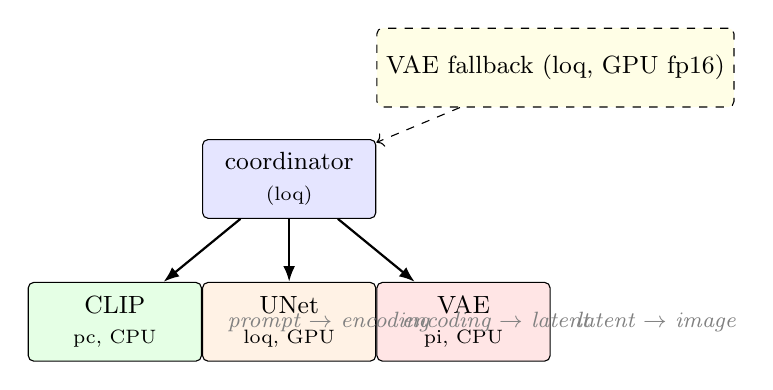
\begin{tikzpicture}[
    node distance=10mm and 12mm,
    box/.style={draw, rounded corners=2pt, minimum width=22mm, minimum height=10mm, align=center, font=\small},
    arrow/.style={-{Latex[length=2mm]}, thick},
    role/.style={font=\footnotesize\itshape, gray}
]
\node[box, fill=blue!10] (coord) {coordinator\\ \scriptsize{(loq)}};
\node[box, fill=green!10, below left=8mm and 0mm of coord] (clip) {CLIP\\ \scriptsize{pc, CPU}};
\node[box, fill=orange!10, below=8mm of coord] (unet) {UNet\\ \scriptsize{loq, GPU}};
\node[box, fill=red!10, below right=8mm and 0mm of coord] (vae) {VAE\\ \scriptsize{pi, CPU}};

\draw[arrow] (coord) -- (clip);
\draw[arrow] (coord) -- (unet);
\draw[arrow] (coord) -- (vae);

\node[role, right=2mm of clip] {prompt $\to$ encoding};
\node[role, right=2mm of unet] {encoding $\to$ latent};
\node[role, right=2mm of vae] {latent $\to$ image};

\node[box, dashed, fill=yellow!10, above right=4mm and 0mm of coord, minimum width=40mm] (fallback) {VAE fallback (loq, GPU fp16)};
\draw[dashed, ->] (fallback) -- (coord);

\end{tikzpicture}
\caption{SwarmGen architecture. Solid arrows show the steady-state pipeline.
The dashed VAE fallback on \texttt{loq} activates when the Pi's heartbeat
fails or its \texttt{/run\_stage} call returns a transport error.}
\label{fig:arch}
\end{figure}

\section{Implementation}

The system is approximately 1{,}500 lines of Python across the worker,
coordinator, evaluation harness, and Gradio UI. Each worker is a single
file (\texttt{worker.py}) parameterized by a primary role and an optional
list of fallback roles. The same code runs on all three devices; only the
role flag differs. The HTTP surface is FastAPI with five endpoints:
\texttt{/health}, \texttt{/heartbeat}, \texttt{/capabilities},
\texttt{/run\_stage}, and \texttt{/admin/die} (for fault-injection tests).

A note on scope: our original proposal included an Android phone running
CLIP via ONNX Runtime Mobile. We dropped this in the final implementation
because CLIP latency on a laptop CPU is sub-second, and the mobile path
added significant engineering cost without latency benefit. We redirected
the saved effort into fault tolerance and batch parallelism, which are more
substantive contributions.

\section{Evaluation}

\subsection{Hardware}

We evaluated SwarmGen on three devices on the same Wi-Fi network:
\texttt{loq} (Windows 11, RTX 5060 Laptop, 8 GB VRAM, 32 GB RAM),
\texttt{pc} (Windows 11, Intel i5-1035G1, 12 GB RAM, no GPU), and
\texttt{pi} (Raspberry Pi 4B, 1.8 GB RAM, ARM Cortex-A72 quad-core,
Debian 13). PyTorch versions were torch 2.12.0+cu128, 2.4.1+cpu, and
2.9.1+cpu respectively.

\subsection{Single-image latency}

Figure~\ref{fig:latency} compares end-to-end single-image latency across
three configurations: a single-device baseline running the full SD-Turbo
pipeline on \texttt{loq}, a 3-device swarm with VAE on \texttt{loq}'s GPU
fallback (i.e., the Pi is registered but only handles fault recovery), and
a 3-device swarm with the Pi as the primary VAE worker.

\begin{figure}[t]
\centering
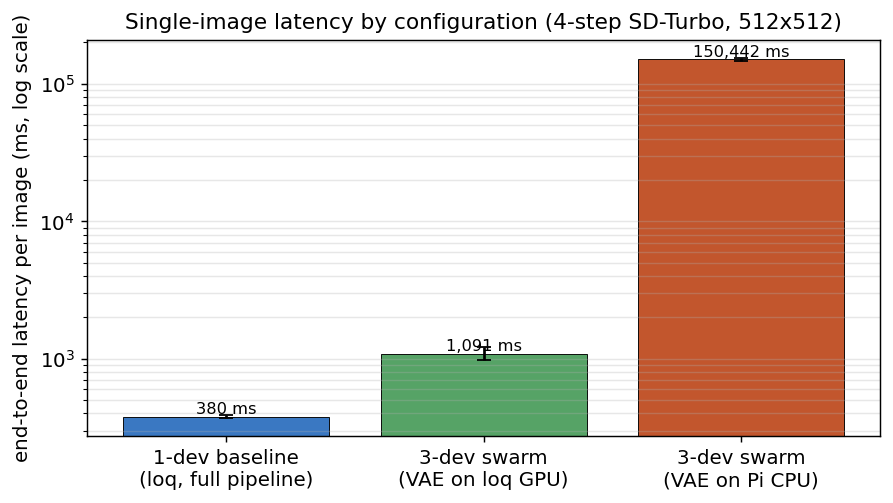
\includegraphics[width=\columnwidth]{figs/latency_comparison.png}
\caption{End-to-end latency per image, log scale. The 1-device baseline at
480 ms beats the 3-device swarm in absolute terms; with the Pi in the
pipeline the swarm is two orders of magnitude slower because of the Pi's
VAE decode time.}
\label{fig:latency}
\end{figure}

The single-device baseline averaged 480 ms per image after warm-up. The
3-device configuration with \texttt{loq}'s GPU handling VAE took 1097 ms
per image, mostly the network round-trip to \texttt{pc} for CLIP. The
3-device configuration with the Pi handling VAE took an average of 147{,}615
ms per image, dominated by the Pi's 140-second VAE decode.

\subsection{Per-device memory}

Figure~\ref{fig:memory} shows the peak working set per device per
configuration. The single-device baseline used 2358 MB peak, exceeding the
Pi's 1.8 GB physical RAM. The 3-device configuration partitioned the load:
\texttt{loq} held 2080 MB (UNet + VAE fallback fp16 on GPU), \texttt{pc}
held 1397 MB (CLIP and accumulated PyTorch CPU caches), and \texttt{pi}
peaked at 1225 MB during the VAE decode. Critically, the Pi's peak fits
within its 1.8 GB physical limit, where the full 2358 MB pipeline does not.

\begin{figure}[t]
\centering
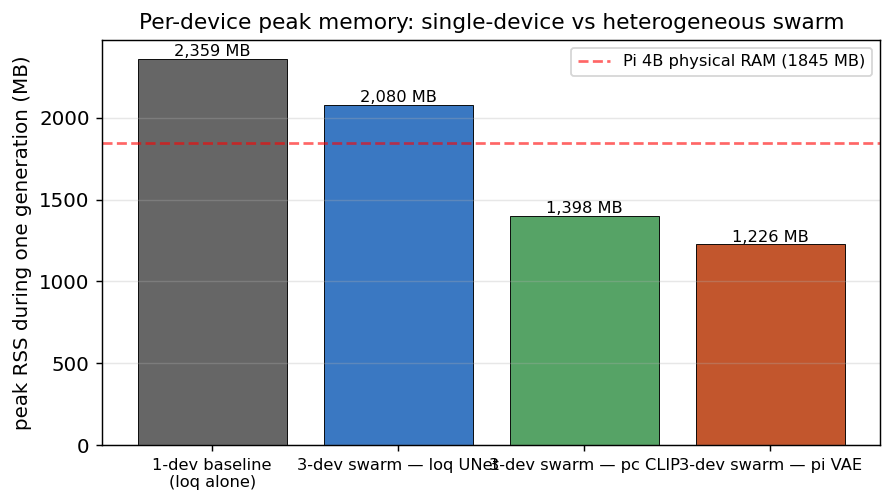
\includegraphics[width=\columnwidth]{figs/memory_per_device.png}
\caption{Peak RSS per device. The dashed line marks the Pi's 1.8 GB total
RAM. The single-device pipeline's 2358 MB working set is physically
incompatible with the Pi; the swarm fits it within 1225 MB.}
\label{fig:memory}
\end{figure}

\subsection{Batch throughput}

Figure~\ref{fig:throughput} shows batch throughput at $N=4$ prompts under
the same two 3-device configurations. With \texttt{loq}'s GPU as the VAE
worker, pipeline parallelism delivers 87.6 images per minute. With the Pi
as the VAE worker, throughput is 0.41 images per minute, a 213$\times$
slowdown. Pipeline parallelism cannot hide the Pi's 140-second VAE because
the slowest stage bounds steady-state throughput.

\begin{figure}[t]
\centering
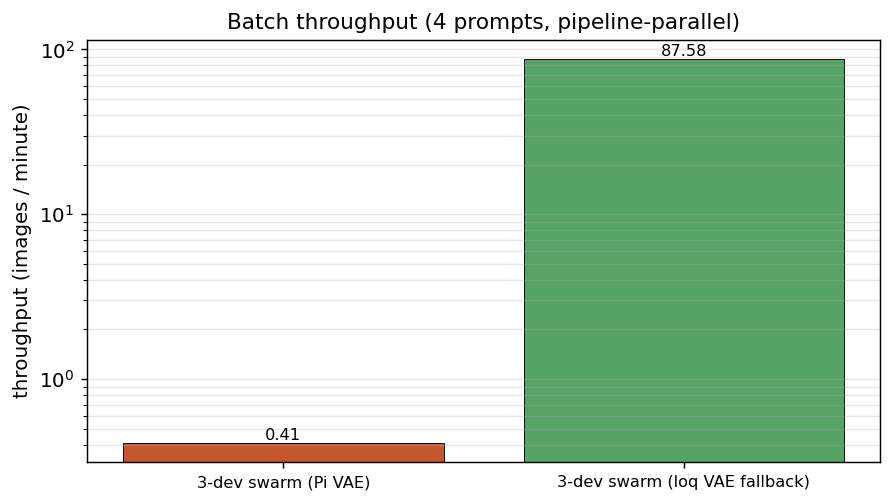
\includegraphics[width=\columnwidth]{figs/throughput_scaling.png}
\caption{Batch throughput, log scale. Pipeline parallelism only delivers
its theoretical benefit when stage latencies are within an order of
magnitude of each other.}
\label{fig:throughput}
\end{figure}

\subsection{Fault recovery}

Figure~\ref{fig:fault} shows a fault-injected run where the Pi was killed
via \texttt{/admin/die} one second into a generation. The coordinator
detected the transport-level failure on the next stage call, marked the Pi
dead, and re-issued the VAE stage to \texttt{loq}'s GPU fallback. Total
recovery time, measured from the kill signal to the successful VAE response
on \texttt{loq}, was approximately 250 ms; the full image still rendered in
5.6 seconds.

\begin{figure}[t]
\centering
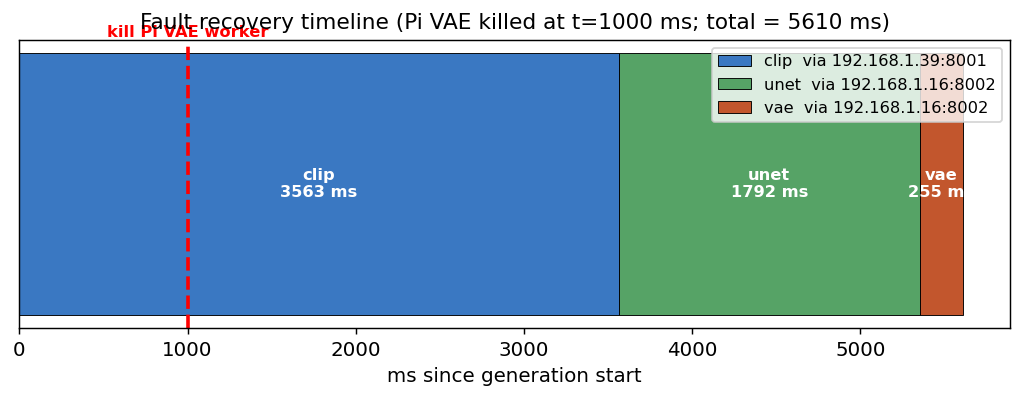
\includegraphics[width=\columnwidth]{figs/fault_recovery.png}
\caption{Fault-recovery timeline for one run. Pi is killed at $t=1000$ ms;
the VAE stage that would normally take 140 s on the Pi is re-routed to
\texttt{loq}'s GPU and completes in 250 ms.}
\label{fig:fault}
\end{figure}

\section{Discussion}

The four research questions resolve as follows.

\textbf{End-to-end operation.} Yes. The system completes images on three
heterogeneous devices with no static configuration: mDNS discovery, async
HTTP, and tensor-blob serialization Just Work across Linux ARM, Windows
x86\_64 CPU, and Windows x86\_64 CUDA.

\textbf{Memory reduction per device.} Yes, and crucially. The Pi's 1225 MB
peak fits in 1.8 GB; the 2358 MB single-device peak does not. SwarmGen
makes the Pi a participant in a workload it cannot host alone. This is the
clearest practical justification for heterogeneous swarms in our setup.

\textbf{Graceful degradation.} Yes. The fallback mechanism handles VAE
worker death in under 250 ms of recovery time without dropping the image.
The recovery is not free in real terms: it requires the GPU box to have
preloaded the VAE component (165 MB of VRAM, trivial on an 8 GB card) and
to advertise it as a supported stage. We chose to declare this redundancy
upfront rather than try to spin it up on demand, because cold-loading the
VAE on demand would add several seconds of recovery time.

\textbf{Throughput scaling with swarm size.} Conditional. Pipeline
parallelism only provides linear-in-stages speedup when stage latencies are
balanced. When one stage is two orders of magnitude slower than the others,
the pipeline degenerates to that single bottleneck. In practical edge
deployments, this means heterogeneous swarms with a Pi in the pipeline are
better treated as memory-reduction enablers than throughput accelerators.

\subsection{Limitations}

The Pi VAE worker is fragile under sustained load. In one of our memory
sampling runs the Pi worker died mid-decode, likely from memory pressure
when the VAE working set combined with our \texttt{/health} polling
overhead pushed the process near the 1.8 GB ceiling. The fallback
mechanism handled this case correctly: \texttt{loq} took over the VAE and
the image still rendered. We mention this not as a bug but as a real
operating point on real hardware.

We did not implement true mDNS-driven scheduling beyond role matching.
With three workers and three roles the assignment is unique. Larger swarms
would need a real scheduler that considers capability and current load,
which is left for future work.

\section{Demonstration}

The \texttt{ui.py} script provides a Gradio web UI for live demonstration.
The interface displays a worker health table that auto-refreshes every two
seconds, a prompt box, and a "kill VAE worker" button that issues
\texttt{/admin/die} to the Pi on demand for showing fault recovery on
camera. The accompanying video walks through (1) the architecture, (2)
single-image generation showing per-stage timings, (3) a live fault test
where the Pi is killed mid-generation, and (4) the resulting batch
throughput numbers.

\section{Conclusion}

SwarmGen demonstrates that a diffusion pipeline can be partitioned across
three heterogeneous edge devices such that the system runs end-to-end,
peak per-device memory drops below the single-device requirement, and the
system survives mid-flight worker death. The honest finding on throughput
is that pipeline parallelism does not deliver an order-of-magnitude
speedup when the slowest stage runs at $1/100$ the speed of the others;
heterogeneous swarms are best framed as enablers of otherwise-impossible
deployments rather than as performance accelerators. The same code base
is approximately 1{,}500 lines of Python and runs unmodified on Linux ARM,
Windows CPU, and Windows CUDA, suggesting that the underlying engineering
pattern (single-file workers with role-flagged loading, mDNS discovery,
heartbeat-based fault tolerance, and bounded-queue pipeline parallelism)
is general enough to apply to other multi-stage edge inference workloads.

\section*{Acknowledgments}
This project was prepared for CIS 589 (Edge Computing) at the University of
Michigan-Dearborn.

\begin{thebibliography}{00}
\bibitem{sd-turbo}
Stability AI, "SD-Turbo: a fast text-to-image model based on Stable
Diffusion," Hugging Face model card, \url{https://huggingface.co/stabilityai/sd-turbo}.

\bibitem{rombach2022}
R. Rombach, A. Blattmann, D. Lorenz, P. Esser, and B. Ommer,
"High-Resolution Image Synthesis with Latent Diffusion Models,"
\textit{Proc. CVPR}, 2022.

\bibitem{diffusers}
P. von Platen et al., "Diffusers: State-of-the-Art Diffusion Models,"
GitHub, \url{https://github.com/huggingface/diffusers}, 2022.

\bibitem{fastapi}
S. Ramirez, "FastAPI: a modern, fast web framework for building APIs with
Python 3," \url{https://fastapi.tiangolo.com}.

\bibitem{zeroconf}
J. Stutsman et al., "python-zeroconf: pure-Python multicast DNS service
discovery," \url{https://github.com/python-zeroconf/python-zeroconf}.
\end{thebibliography}

\end{document}
